%%%%%%%%%%%%%%%%%%%%%%%%%%%%%%%%%%%%%%%%%%%%%%%%%%%%%%%%%%%%%%%%%%%
%%% Documento LaTeX 																						%%%
%%%%%%%%%%%%%%%%%%%%%%%%%%%%%%%%%%%%%%%%%%%%%%%%%%%%%%%%%%%%%%%%%%%
% Título:		Introducción
% Autor:  	Ignacio Moreno Doblas
% Fecha:  	2014-02-01, actualizado 2019-11-11
% Versión:	0.5.0
%%%%%%%%%%%%%%%%%%%%%%%%%%%%%%%%%%%%%%%%%%%%%%%%%%%%%%%%%%%%%%%%%%%
% !TEX root = A0.TFG.tex

\chapterbegin{Tecnología a usar}




\section{Tecnología a usar}
\label{sec:tecnologiaUsar}






Para el desarrollo de este proyecto se necesita un dispositivo de realidad virtual simple y compacto, que sea fácil de transportar y que no requiera de mucha preparación para utilizarlo, ya que será usado por personas mayores o con movilidad limitada y es necesario que el dispositivo no suponga ningún impedimento a la hora de utilizarlo. Por esto se han descartado los dispositivos con cables que los conectan a un ordenador o aquellos que necesitad de sensores externos y que complicarían la instalación y uso.

Además de cumplir estas características, es necesario que sea una plataforma soportada por algún motor de videojuegos de los que están preparados para desarrollar aplicaciones de realidad virtual.

Los dos principales cascos de RV que cumplen estas características son el Oculus Go y el Meta Quest 2 (véase figura \ref{fig:TU_oculusQuest}). Ambos dispositivos son inalámbricos y funcionan con batería. Cuentan con una distribución especializada de Android sobre la que se ejecutan los juegos. Sin embargo, Oculus Go tiene unas especificaciones inferiores y la capacidad de seguimiento del casco y los mandos no es tan buena.

\begin{figure}
  \centering
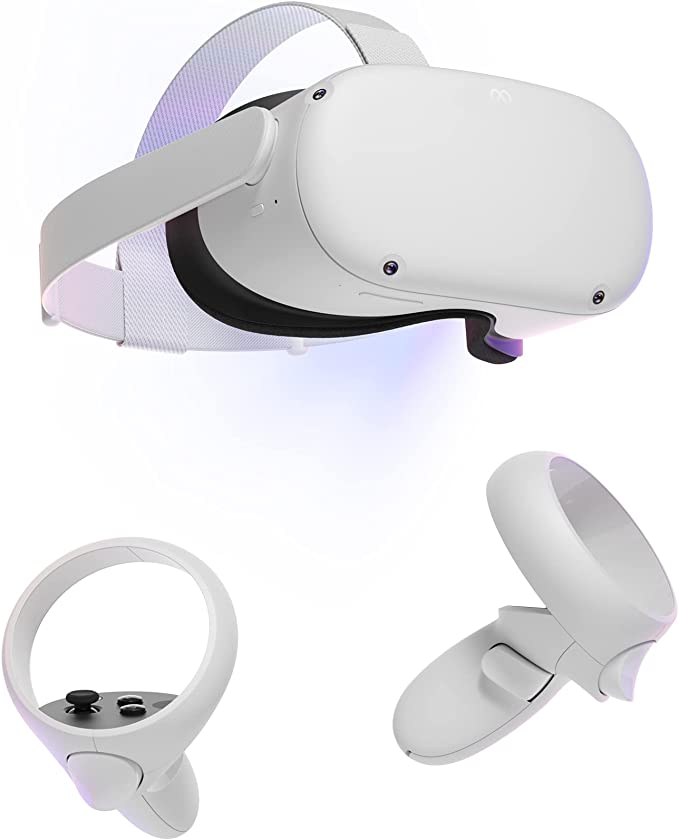
\includegraphics[width=0.5\textwidth]{03.EstudioProblema/03.TecnologiaAUsar/00.Figuras/04.meta_quest_2.jpg}
    \caption{Meta Quest 2. \cite{EA_img_oculusQuest}}
    \label{fig:TU_oculusQuest}
\end{figure}

Ya que el dispositivo será utilizado por personas mayores, es necesario hacer la experiencia lo más sencilla posible en el lado técnico, por lo que un seguimiento excelente de los mandos es necesario para evitar problemas y confusión en las personas.

%Por estos motivos, se escoge Meta Quest 2 como plataforma sobre la que desarrollar este proyecto.
Por estos motivos, se define Meta Quest 2 como plataforma ideal para este desarrollo. Sin embargo, a fecha del comienzo de este proyecto, no se dispone de ningún dispositivo de este tipo y se desconoce si se podrá disponer de él. Por lo que se comienza este trabajo utilizando unas HTC Vive, el dispositivo desarrollado conjuntamente entre Valve y HTC. Estas gafas, aunque potentes, requieren estar conectadas permanentemente a un ordenador y usan estaciones externas para el seguimiento de los movimientos del jugador. Durante el desarrollo del proyecto se consiguió acceso a un set de Meta Quest 2, por lo que se cambia el dispositivo durante el desarrollo. A pesar de generar trabajo extra, este cambio permite trabajar con bibliotecas más modernas y ofrece un resultado mucho más adecuado a las características de este proyecto como se ha definido en el inicio de esta sección.


Para desarrollar el juego es necesario también un motor de videojuegos, en este caso, tanto Unreal Engine 4 como Unity son compatibles con Meta Quest 2 y HTC Vive. En este caso se va a elegir utilizar Unity (figura \ref{fig:TU_interfazUnity}) ya que tiene gran cantidad de documentación disponible sobre RV, está muy optimizado para la plataforma Android y además tiene paquetes y bibliotecas que permiten trabajar de manera más sencilla con Meta Quest 2 y HTC Vive.

\begin{figure}
  \centering
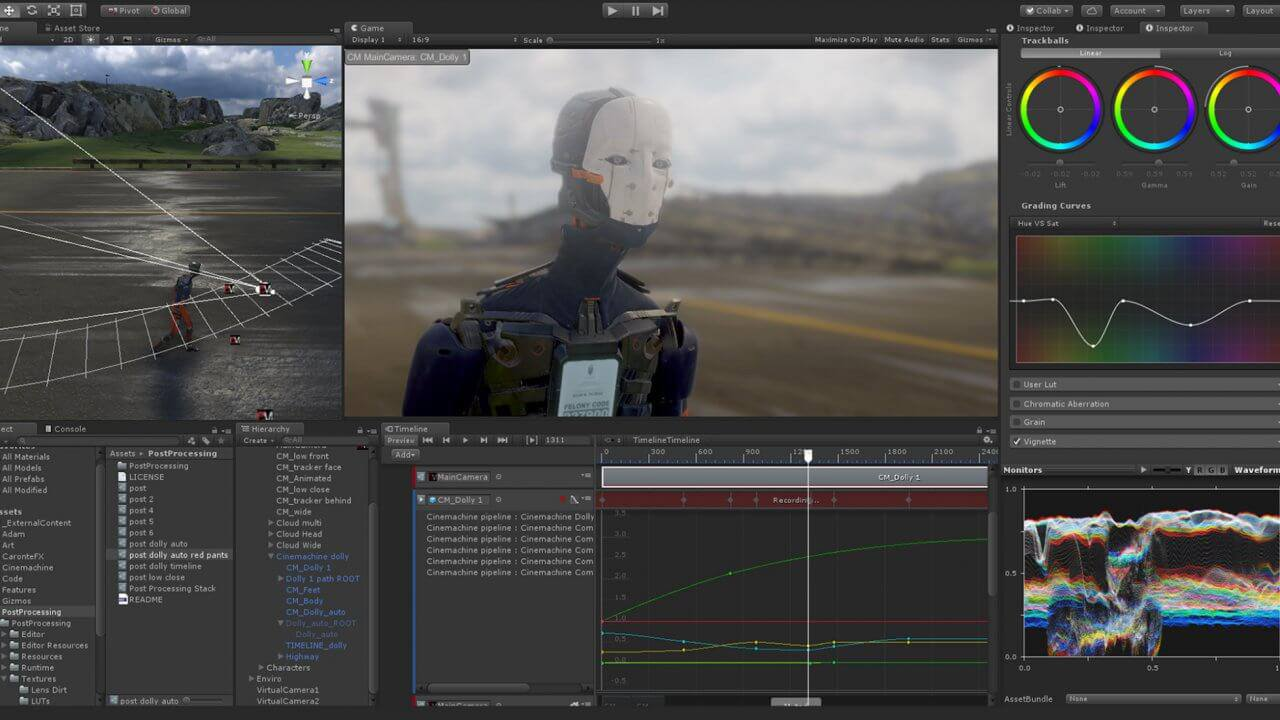
\includegraphics[width=0.8\textwidth]{03.EstudioProblema/03.TecnologiaAUsar/00.Figuras/02.interfaz_unity.jpg}
    \caption{Interfaz de Unity. \cite{EA_img_interfazUnity}}
    \label{fig:TU_interfazUnity}
\end{figure}

La principal biblioteca que apoyará el desarrollo del proyecto es VRTK 4. Es una compilación de diferentes scripts que permiten la fácil implementación de mecánicas indispensables en un videojuego de realidad virtual:

\begin{itemize}
	\item{Locomoción.}

	\item{Interacciones con objetos virtuales (coger, soltar, empujar…).}

	\item{Interacción con una interfaz dentro del espacio virtual.}
	
	\item{Controladores como botones y palancas.}

\end{itemize}


Unity es un programa con un funcionamiento modular, lo que significa que pueden agregarse paquetes de funcionalidad de manera sencilla desde su tienda integrada: Asset Store (vease figura \ref{fig:TU_assetStore}). Todos los paquetes necesarios para el desarrollo de este proyecto están disponibles en la Asset Store y se pueden descargar de forma directa desde Unity.

\begin{figure}[H]
  \centering
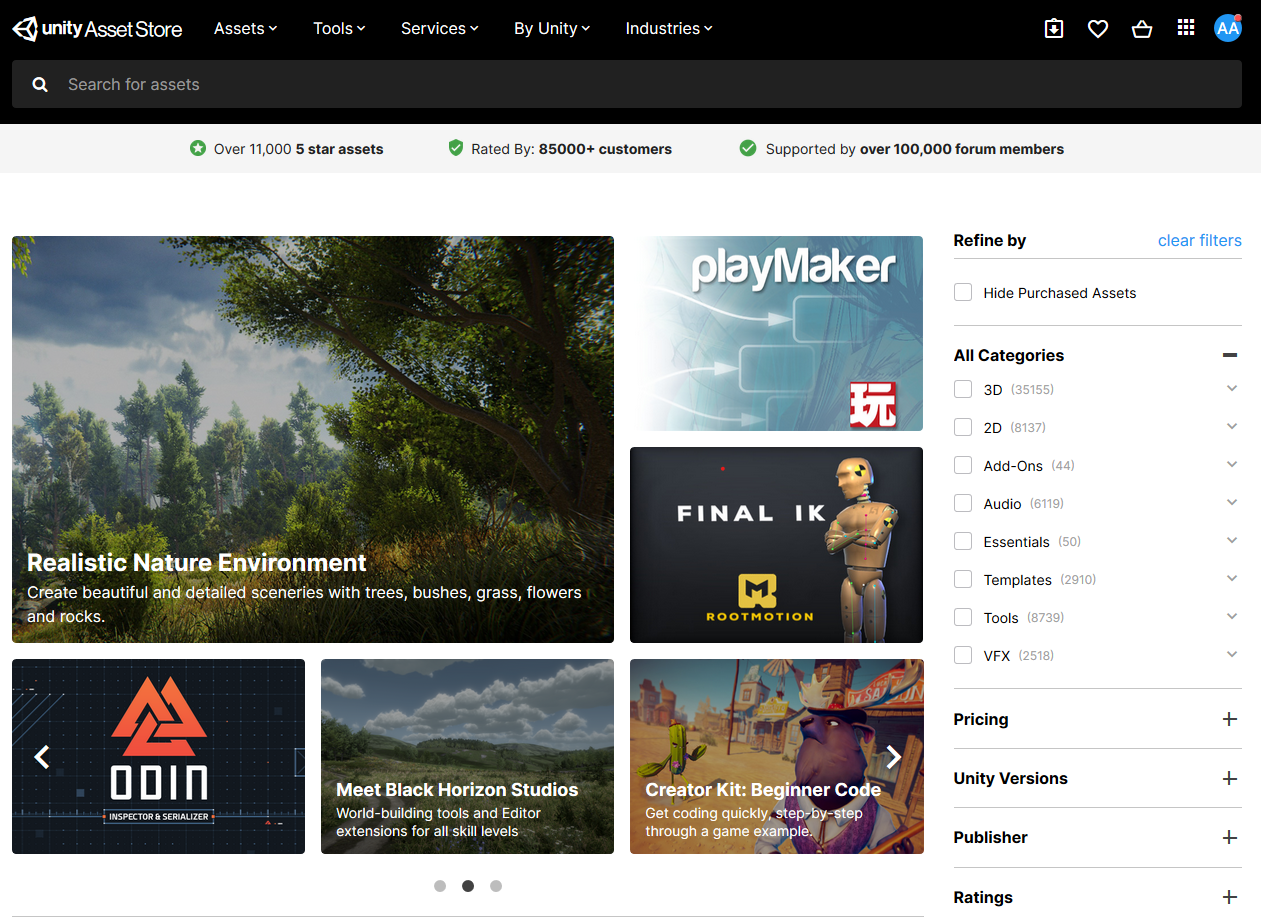
\includegraphics[width=0.8\textwidth]{03.EstudioProblema/03.TecnologiaAUsar/00.Figuras/03.asset_store.png}
    \caption{Portada de la Asset Store.}
    \label{fig:TU_assetStore}
\end{figure}



Adicionalmente, trabajar con VRTK permite cierta abstracción de la plataforma final del videojuego, ya que es compatible tanto con los dispositivos de Meta, como con todos aquellos cascos de RV compatibles con SteamVR, el sistema de RV de la empresa Valve. Esto permitirá que, una vez finalizado el proyecto, se pueda extender fácilmente para funcionar también con el resto de los dispositivos VR actuales y, posiblemente, futuros.


\chapterend